\textbf{Atletas que hayan participado en más de 1 disciplina.}\vspace{.3cm}

Podemos consultar toda la información de los atletas que hayan participado en más de una disciplina mediante la tabla Participa en la base de datos, por lo que haremos un join entre ambas, luego vamos a contar aquellos que tengan asociado más de un IDDisciplina diferente. 

La consulta quedaría así:
\begin{center}
    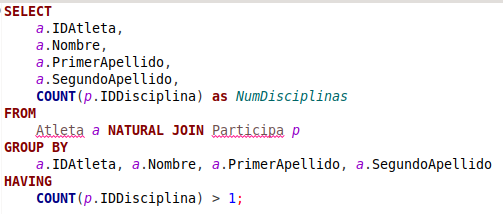
\includegraphics[width=10cm]{resources/consulta3.png}
\end{center}
Nótese que añadimos una columna donde se indican en cuántas disciplinas participan los atletas

El resultado será:
\begin{center}
    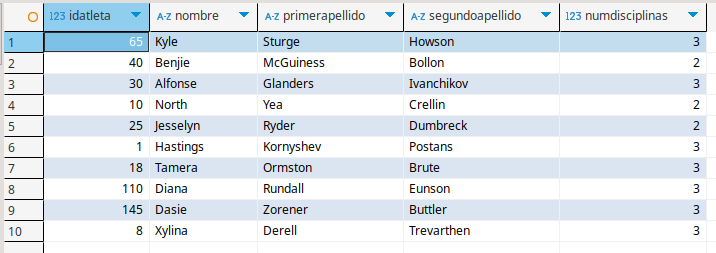
\includegraphics[width=15cm]{resources/consulta3.1.png}
\end{center}


